\documentclass[letterpaper,twocolumn,10pt]{article}
\usepackage{usenix,epsfig,url}
\usepackage{graphicx}
\usepackage{multirow}
\usepackage{rotating}
\usepackage[font={small,it}]{caption}
\usepackage{url} 
\urlstyle{sf}

\begin{document}

\title{\Large \bf Log-Structured Cache: Trading Hit-Rate for Storage Performance
  (and winning) in Mobile Devices}

% \author{
%   {\rm Abutalib Aghayev, Peter Desnoyers}\\
%  Northeastern University
% }
\date{}
\maketitle

\thispagestyle{empty}

\subsection*{Abstract}
Browser caches are typically designed to maximize hit rates---if all other
factors are held equal, then the highest hit rate will result in the highest
performance. However, if the performance of the underlying cache storage
(i.e. the file system) varies with differing workloads, then these other factors
may in fact not be equal when comparing different cache strategies.

Mobile systems such as smart phones are typically equipped with low-performance flash
storage, and suffer severe degradation in file system performance under
sufficiently random write workloads. A cache implementation which performs
random writes will thus spend more time reading and writing its cache, possibly
resulting in lower overall system performance than a lower-hit-rate
implementation with higher storage performance.

We present a log-structured browser cache, generating almost purely sequential
writes, in which cleaning is efficiently coupled with cache
eviction. We evaluate an
implementation of this cache for the Chromium browser on Android, using
captured user browsing traces, comparing 
its performance to the existing Chromium implementation.

We achieve a ten-fold performance improvement in basic cache operations (as
measured on a Nexus 7 (2012 version) tablet), while in the worst measured case
decreasing hit rate by less than 1\% (from 37.9\% to 36.1\%) and more
typically by less than 0.5\%. For network
bandwidths of 350\,Kb or higher the increased cache performance will
more than make up for the decrease in hit rate; the effect is more
pronounced with smaller object sizes which may be typical of mobile
browser usage.

\section{Introduction}

The use of mobile computing devices like smartphones and tablets is growing at a
remarkable speed, and analysts are predicting mobile users surpassing desktop
users within a year~\cite{ingram10}.  Mobile devices are being equipped with ever-faster
CPUs and significant amounts of RAM, yet their performance lags far
behind that of even low-end desktops. While part of this disparity
in performance is due to slower networks and CPU, recent work by Kim
et al.~\cite{kim12} has shown that flash storage may be the primary
bottleneck in many mobile  applications.

Mobile devices typically contain some amount of \emph{on-board} or
non-removable flash storage, as well as provision for removable storage devices
such as MicroSD cards. The experiments reported by Kim et al. examine
removable storage; however their results are likely  to apply to on-board
storage as well. This is due to the widespread use of eMMC (Embedded Multi-Media
Card) devices for on-board flash---these are these are essentially MicroSD cards
in a soldered package. Like a MicroSD card, they typically rely on an 8-bit
micro-controller for internal processing, using simple algorithms which offer
adequate performance for sequential applications like music and photography, but
which may degrade catastrophically when handling the random access
patterns generated by complex applications.

One such complex application is a web browser.  Browsers are by far the most
commonly-used application on desktops, and are becoming so on tablets and
smartphones; they use disk (or flash) storage as a persistent cache for
retrieved objects for possible re-use, greatly speeding up the loading of some
web pages.  An average web page contains about 50
resources~\cite{google-web-metrics}, therefore, even moderate browsing activity
results in large numbers of individual read and write operations.

Browser caches present an unusually write-heavy workload, as typical
hit rates for an individual cache are below 50\%---i.e. for
every hit which results in a read from the cache, there is at least one
miss, resulting in a write. As long as write performance is high enough
this need not impact performance, as writes may be performed in
the background while a newly-fetched object is being displayed;
however overall performance will suffer if cache writes become a
bottleneck. 

Modern browsers like Chromium~\cite{chromium} or
Firefox~\cite{Firefox} employ LRU or LFU eviction in their caches to
maximize hit rate. This results in highly random write patterns;
although the operating system may be able to coalesce some of these
writes, the resulting write pattern is still very non-sequential,
resulting in poor file system performance on  eMMC-equipped mobile
devices we have tested. Not only are writes very slow under these
conditions, but the lack of command queuing on the underlying flash
storage results in high read latency due to interference from writes.

Under these circumstances, the cache resulting in optimal application
performance may not be the same as the one resulting in optimal hit
rate. In fact we argue that this trade-off is fundamental: any
eviction algorithm based purely on attributes of the cached objects
(e.g. LRU) is going to generate highly non-sequential writes when
operating with an entirely full cache, and (under reasonable
assumptions) any mechanism to reduce this randomness will require
reducing the effective cache size, thus reducing the expected hit rate.

We present an implementation and analysis of a cache designed to maximize write
throughput to flash storage, at the cost of a small decrease in hit rate. The
cache is structured much like a log-structured file system~\cite{rosenblum92},
dividing storage into large \emph{segments} which are written
sequentially, relying on the file system to buffer data and perform
large sequential writes. 
Once filled, segments are immutable and cannot be reused until they are
\emph{cleaned}; cache eviction occurs as part of this cleaning
process, and results in much higher cleaning performance than is
typical in log-structured file systems.

The contributions described in this paper are as follows:

\begin{itemize}

  \item We present a design and rationale for a log-structured cache optimized
    for write performance on low-end flash media.

  \item We present experimental results showing a nearly ten-fold improvement in
    read and write latency for cache operations on a mobile platform when
    compared to the existing Chromium cache.

  \item Using real browsing traces collected over a period of two months, we
    compare our cache to the existing cache.  The
    reduction in hit rate is no more than 1\% (37.9\% to 36.9\%) across
    the traces and cache sizes evaluated, and typically between 0 and 0.5\%.

\end{itemize}

\section{Overview and Rationale}
Although today's smart phones run general purpose operating systems on CPUs as
powerful as desktop machines of several years ago, storage systems on these
devices are far less powerful than those on typical desktops or laptops.
Almost all Android devices on the market appear to use eMMC~\cite{emmc_2010}
storage, essentially a soldered-down version of a MicroSD card.  Where
desktop and laptop SSDs use 32-bit micro-controllers with megabytes of memory to
run the algorithms which translate operating system requests to flash
operations, these low-end devices may rely on a 8-bit microcontroller with less
than 10\,KiB of RAM.

\subsection{Mobile storage performance}

As an example, in Figure~\ref{fig:seq-throughput} we see sequential read and
write throughput for direct I/O (i.e. un-cached) requests to a 16\,MiB file on a
Nexus 7 tablet running the Android operating system. Write bandwidth
is less than 1\,MB/s for write sizes under 8\,KiB, and does not reach
full bandwidth until 4\,MiB. In Figure~\ref{fig:rnd-throughput} we see
throughput for small random reads and writes; write througput is
17\,KB/s for 512-byte writes, rising to 190\,KB/s for 4096-byte
writes. 

\begin{figure}[t]
  \begin{center}
    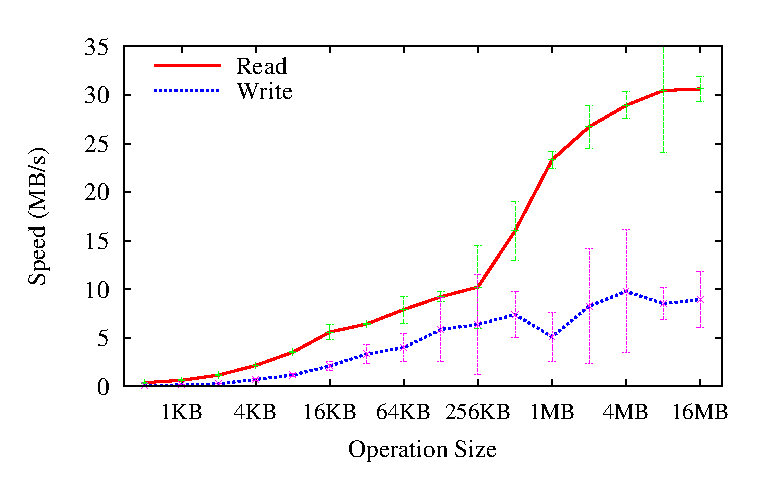
\includegraphics[width=1.04\columnwidth]{graphs/seq-throughput}
  \end{center}
  \caption{Sequential I/O throughput of the eMMC found on Nexus 7.}
  \label{fig:seq-throughput}
\end{figure}

\begin{figure}[t]
  \begin{center}
    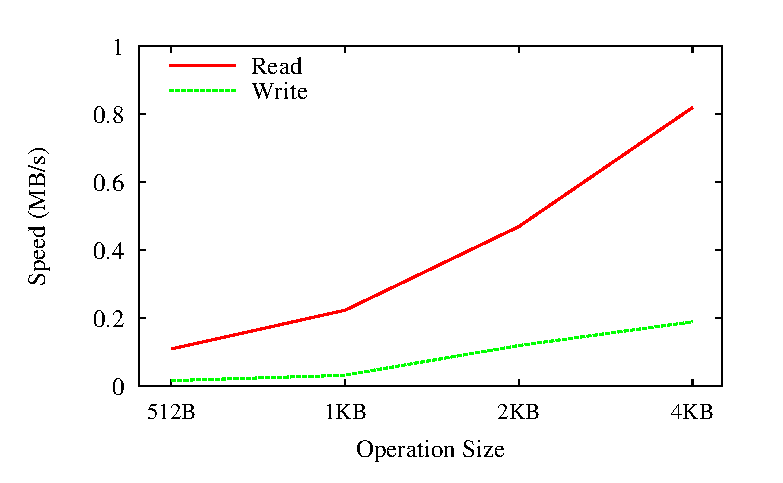
\includegraphics[width=1.04\columnwidth]{graphs/rnd-throughput}
  \end{center}
  \caption{Random I/O throughput of the eMMC found on Nexus 7.}
  \label{fig:rnd-throughput}
\end{figure}

These performance measurements are comparable to what was observed in the
recent work of Kim et al.~\cite{kim12} which measured the performance of
external storage (MicroSD cards) on a Nexus One
phone.  In both cases, performance for small random writes was found
to be virtually unusable.  This is a known artifact of the flash translation
algorithms used on controllers with limited memory~\cite{Kim2002:FTL}, which
with modern flash chips may suffer 128$\times$ or worse decrease in throughput for
random writes~\cite{boboila_performance_2011}.

\subsection{Log-structured cache}
As can be seen in the Figure~\ref{fig:galaxy-nexus-seq}, read performance on
these devices is fairly high --- even for reads as small as 4KB --- while large
sequential writes must be used to achieve high write performance.
The combination of these storage characteristics and the write-heavy load
offered by a low hit-rate cache suggests the use of a log-structured,
write-optimized approach to cache storage similar to Rosenblum and Ousterhout's
Log-structured File System~\cite{rosenblum92}.

Log-structured file systems divide the storage into large fixed sized segments,
only one of which (the \emph{write frontier}) is written to at a time.  Writes
are buffered in memory until a full segment can be written to disk.  Updates to
existing data are written to the write frontier and cause the overwritten data
(living in some previous segment) to become obsolete.  When the number of free
segments drops below a certain threshold, a cleaning process chooses segments to
be compacted.  Any remaining live data from these segments is copied to the
write frontier, making these segments available for reuse.

This process of compacting live data in a log-structured file system is known as
~\emph{segment cleaning}.  Finding an efficient segment cleaning algorithm has
been the most challenging part of the log-structured file systems.  Much
research has been devoted to it, with the best implementations still suffering serious
performance degradation under certain scenarios~\cite{seltzer93}.

The design of our cache is similar to the design of the log-structured file
system.  A large preallocated file is used instead of a block device and is
divided into fixed sized segments, which are written sequentially. The
cleaning process is simplified substantially, however, by taking
advantage of the volatile nature of cached data. Segments are selected
for cleaning in FIFO order, and within each segment we track which
objects have been used since the segment was written. Those objects
are copied back to the write frontier, much as pages with the A bit
set are skipped in the CLOCK replacement algorithm \cite{corbato_paging_1969}.

\subsection{Hit rate vs. sequentiality trade-offs}

Our log-structured cache performs purely sequential writes, but at the
cost of a hit rate that is slightly lower than that of LRU or the
existing Chrome browser cache. We present an informal argument that
LRU and similar algorithms when using demand eviction will generate
writes which are randomly and uniformly distributed across the storage
space, and that any modification which increases the sequentiality of
these writes will necessarily involve some decrease in hit rate.

We assume a cache holding S objects, where a new object is inserted by
choosing the least-recently-used object and over-writing it. In the
steady state there will be no correlation between the location of
an item in storage and its most recent use time; the resulting writes
will thus be uniformly distributed over the S storage locations.
In this situation it is unlikely that buffering in the file system
will do much to increase sequentiality of write operations.
If $M$ objects are buffered in memory before writing, $M<S$,
then the probability that an individual write cannot be merged with
the following one is $\frac{S-M}{S}$, and the mean write length will
be $\frac{S}{S-M}$; i.e. less than 2 for $M<\frac{S}{2}$.

To increase write sequentiality it is necessary that
there be a choice of locations into which a new object will be
written. This may be done in one of two ways: (a) a different object
may be chosen for eviction, or (b) multiple free locations may be
maintained.

Option (a) results in eviction of an object other than that identified
as the best candidate for eviction; since this is done based on
information unrelated to the request stream, its effect on hit rate
should be negative for any replacement strategy better than random.

For alternative (b), assume we reserve $k$ locations, either
permanently or on average via a high/low-water mark method of
eviction, resulting in a cache which holds $S'=S-k$ objects. Since hit
rate is a non-decreasing function of $S$ for stack algorithms such as
LRU, and expected hit rate is an increasing function of cache size for
any useful replacement algorithm, the result is a decrease in hit rate
when compared to the original cache holding $S$ objects. 

\begin{figure}
\centering
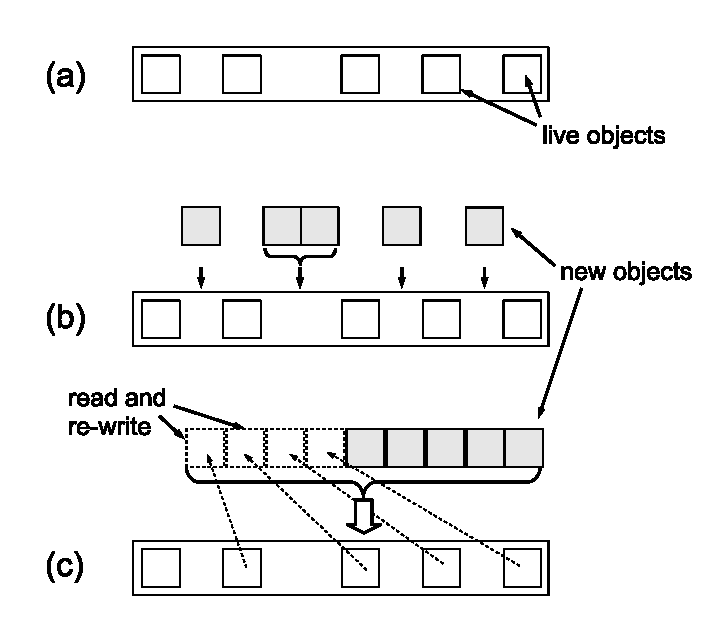
\includegraphics[width=\columnwidth]{graphs/re-write}
\caption{Writing new entries to cache, without and with compaction.}
\label{fig:rewrite}
\end{figure}

If some number of free locations are reserved, write sequentiality may
be further increased by performing a larger number of writes. In
Figure \ref{fig:rewrite}(a) we see a section of cache with free and in-use
locations; if the free locations are written directly, as shown in
Figure \ref{fig:rewrite}(b), the result is four individual writes.
However if we compact storage by reading and re-writing in-use data,
in Figure \ref{fig:rewrite}, the total volume of data written increases, but
it may be written by a single sequential operation.

In our log-structured cache we take advantage of both additional free
space, of up to an entire segment, as well as additional writes for
copying recently-used objects during cleaning. The result is an
algorithm which generates fully sequential writes, while achieving hit
rates nearly as high as those for a widely-used LRU-like algorithm
(the existing Chrome cache) at the cost of a very small increase in write
traffic. (Due to the elimination of internal write amplification from
random writes, wear on the flash device is still expected to be much
lower than for the original cache algorithm.)

\section{Log-Structured Cache Design}

Our log-structured cache was implemented and evaluated in Chromium, the
open-source browser from Google.  This decision placed certain constraints on
our design, due to the cache API and overall architecture of Chromium.
In this section we first describe the relevant aspects of the Chromium
caching architecture, and then the structures and operation of the
log-structured cache.

\subsection{Chromium's cache architecture}

Chromium's cache is implemented in two layers.  At the lower layer there is a
generic object cache \emph{backend}, that can store \emph{entries} consisting of
a fixed number of \emph{streams}, each of arbitrary size.  C++ definitions for
the key portions of the API for this layer are shown In Figure~\ref{cache-api};
this interface is used for storage and retrieval by higher-layer caching
components in Chromium.

The primary user of this interface is the \emph{HTTP cache}, used to store most
webpage objects. The HTTP cache uses two streams for each object cached; one
stream holds the HTTP metadata such as content-type and last-modified time,
while the other holds the object itself.  This two-layer design allows the same
lower-layer cache backend and replacement policy implementation to be used for
multiple higher-layer caches, each with different semantics.  Examples of
higher-layer caches are the \emph{media cache} and the \emph{HTML5 AppCache},
both with different caching semantics; we do not consider them in this work.

In order to achieve high performance and fast user response, almost every
internal API in Chromium is asynchronous, through the use of callback functions
as shown in Figure~\ref{cache-api}.  Function calls return immediately and the
return value determines whether the operation has completed; if not, a task is
posted to a dedicated \emph{cache thread} and a callback invoked at some time in
the future to indicate a completed task.  

\begin{figure}[h]
{\small
\begin{verbatim}
// Backend class methods
int CreateEntry(const std::string& key,
                Entry** entry,
                const CompletionCallback& cb) = 0;
int OpenEntry(const std::string& key,
              Entry** entry,
              const CompletionCallback& cb) = 0;

// Entry class methods
int ReadData(int stream_index,
             int stream_offset,
             IOBuffer* buf,
             int buf_len,
             const CompletionCallback& cb) = 0;
int WriteData(int stream_index,
              int stream_offset,
              IOBuffer* buf,
              int buf_len,
              const CompletionCallback& cb) = 0;
void Doom() = 0;  // Mark entry for deletion.
void Close() = 0;  // Release a reference to entry.
\end{verbatim}
}
\caption{Chromium Cache Backend API.}
\label{cache-api}
\end{figure}

\subsection{The new backend}

The log-structured cache implementation stores data in a single large file,
which as shown in Figure~\ref{fig:storage} is divided into large
fixed-size segments.  The segment size is chosen to be much larger than the average cache
entry, and to be larger than the cleaning unit of the flash device (typically
4\,MiB for eMMC devices we have seen).  Since the cache operates above the file
system it is not possible to align segments with underlying storage boundaries;
however it is typically allocated sequentially by the file
system\footnote{This is confirmed by \texttt{blktrace} measurements in
  Figure \ref{fig:blktrace:flash}, below.}.

\begin{figure}[t]
  \begin{center}
    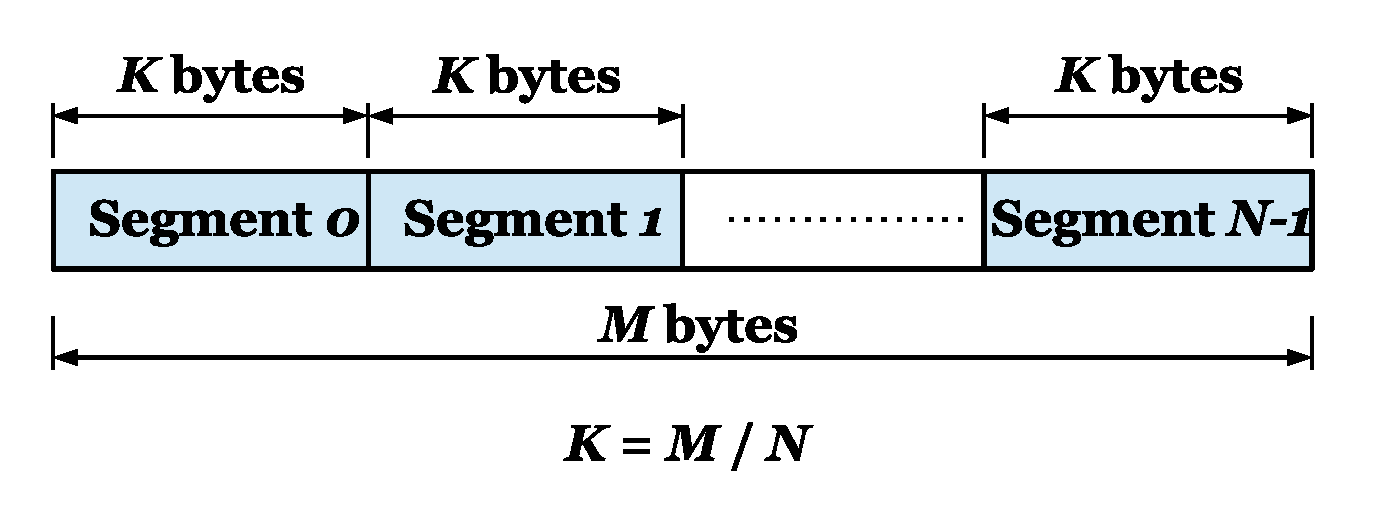
\includegraphics[width=\columnwidth]{graphs/storage}
  \end{center}
  \caption{Log-structured cache view of the storage.}
  \label{fig:storage} 
\end{figure}

Each segment holds multiple entries, followed by a footer or \emph{segment
  summary} holding offsets to each entry in the segment, for more efficient
scanning at cleaning time.  An entry consists of a header, followed by a key
(e.g. URL), followed by one or more streams. Figure~\ref{fig:segment} shows the
entry layout when the log-structured cache backend is used by an HTTP cache.
Internally, we do not distinguish the key from the other streams and consider it
to be just another stream.  The header is of fixed size and holds the size of
each stream.

The segment summary has a fixed number of slots and stores the offsets of every
entry that was written to the segment; entries do not span multiple segments.
The segment size thus determines the maximum size of an entry that can be
inserted into the cache, and the number of entries that can be stored in a
segment is determined by the number of slots in the segment summary.  Entries
larger than a segment are stored as separate files on disk, just like the
current cache does.  The segment summary is sized assuming a mean entry size of
4\,KiB, a conservative value based on trace data shown in Figure~\ref{fig:log-size-dist}.

\begin{figure}[t]
  \begin{center}
    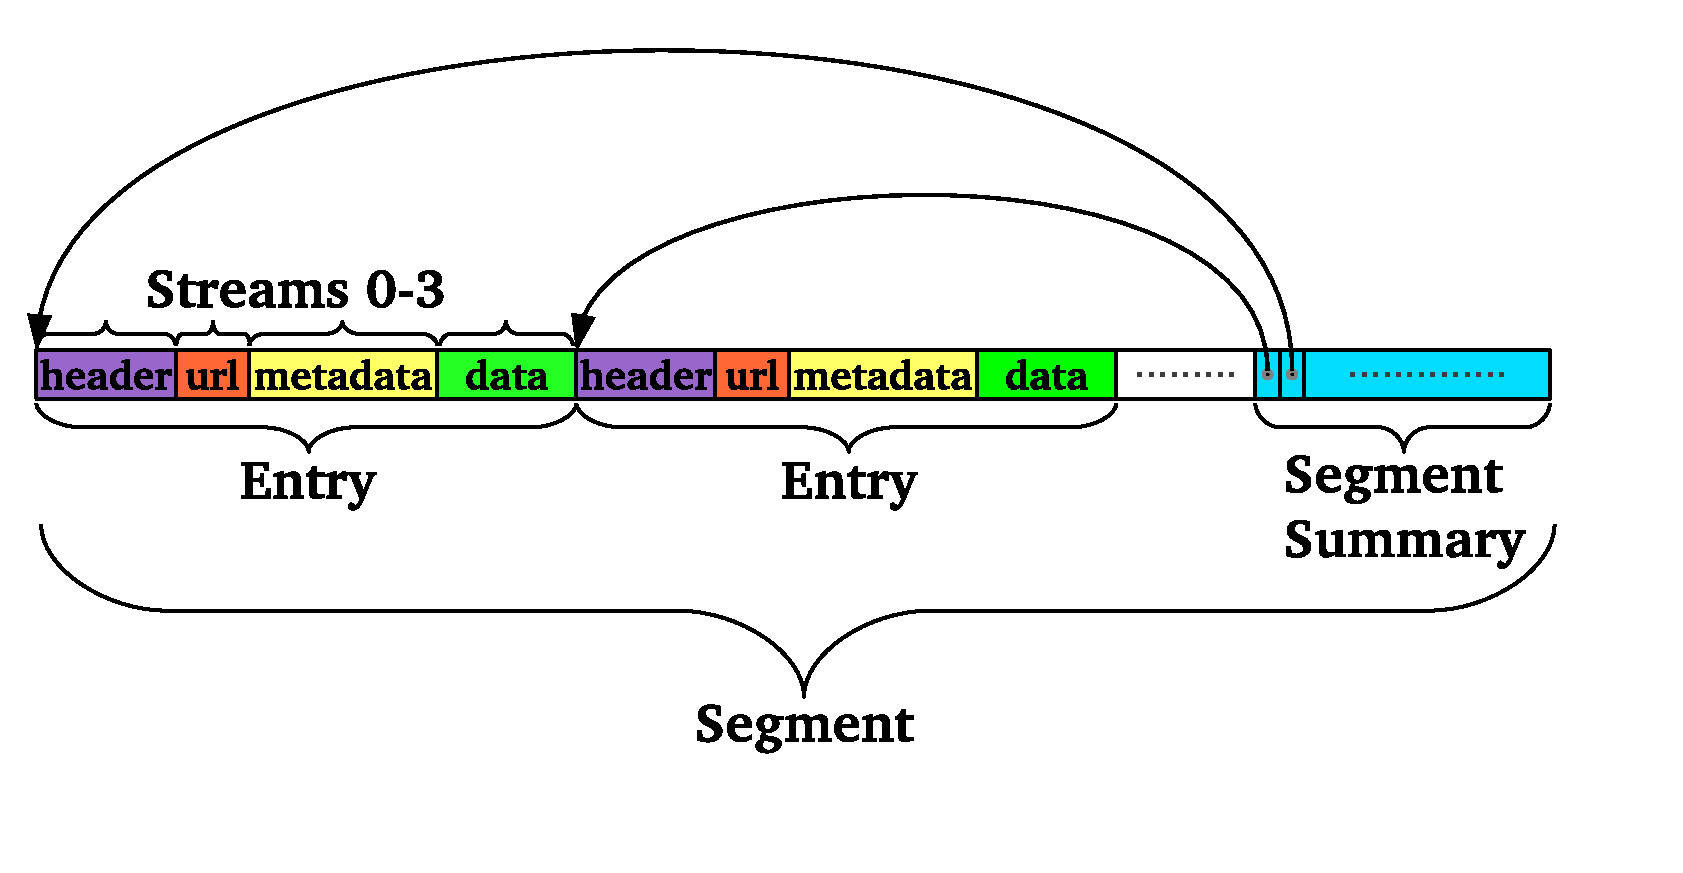
\includegraphics[width=\columnwidth]{graphs/segment}
  \end{center}
  \caption{Contents of a Segment.}
  \label{fig:segment} 
\end{figure}

\subsubsection{The Index}
In addition to storing entries, we also store the cache index, which maps the
hash of the key (for the HTTP cache, the URL) to the corresponding entry's
location in the file, as shown in Figure~\ref{fig:update}.  The index is very
small in comparison to the cache storage, and is updated on every new entry
insertion.  It is thus kept in memory as a memory-mapped file, which would only
be written back to storage under memory pressure or on browser exit. (If the
index is corrupted by a power failure, the entire cache can be emptied).  In our
prototype implementation the in-memory hash structure is not mapped to a file.

\subsubsection{Insert}
Inserting an entry into the cache backend involves a few steps.  Once the key of
the entry to be cached is known, the high-level cache calls \emph{CreateEntry}
member function of the \emph{Backend} object, which upon success returns an
\emph{Entry} handle.  As the data is received from the network, the streams of
the entry are populated via \emph{WriteData} call.  The entry is buffered in
memory until \emph{Close} is called.  After \emph{Close} is called, the entry is
written to the current segment and its location in file is written to index as
well as the segment summary.  Segment summary of the current segment is buffered
in memory and is not written until the segment is full, resulting in sequential
fill of the segment.

\subsubsection{Open}
A cache lookup from the upper layer results in a call to \emph{OpenEntry}, which
attempts to locate an existing entry with a specified key and open it for
reading.  Given the key, it calculates the hash and uses the index to find the
location of the entry within the file.  Once found, the header is read and the
offsets of the streams can be calculated and streams can be read.

\subsubsection{Delete}
If the upper layer determines after creating an entry that it should not
actually be cached, it may mark it for deletion by calling \emph{Doom}.  When
\emph{Close} is called, the in-memory entry is destroyed rather than being
written to storage.  To delete a previously inserted entry, it must be opened
(\emph{OpenEntry}), and then may be marked for deletion (\emph{Doom}), and
closed (\emph{Close}).  In this case the index is updated, and the space
occupied by the entry will become usable when the segment is cleaned.


Note that deleting an entry is performed by the upper layer, and is used when a
particular object \emph{must} be removed from cache; in contrast, eviction is
performed by the cache backend, and selects objects which \emph{may} be removed
from cache.

\begin{figure}[t]
  \begin{center}
    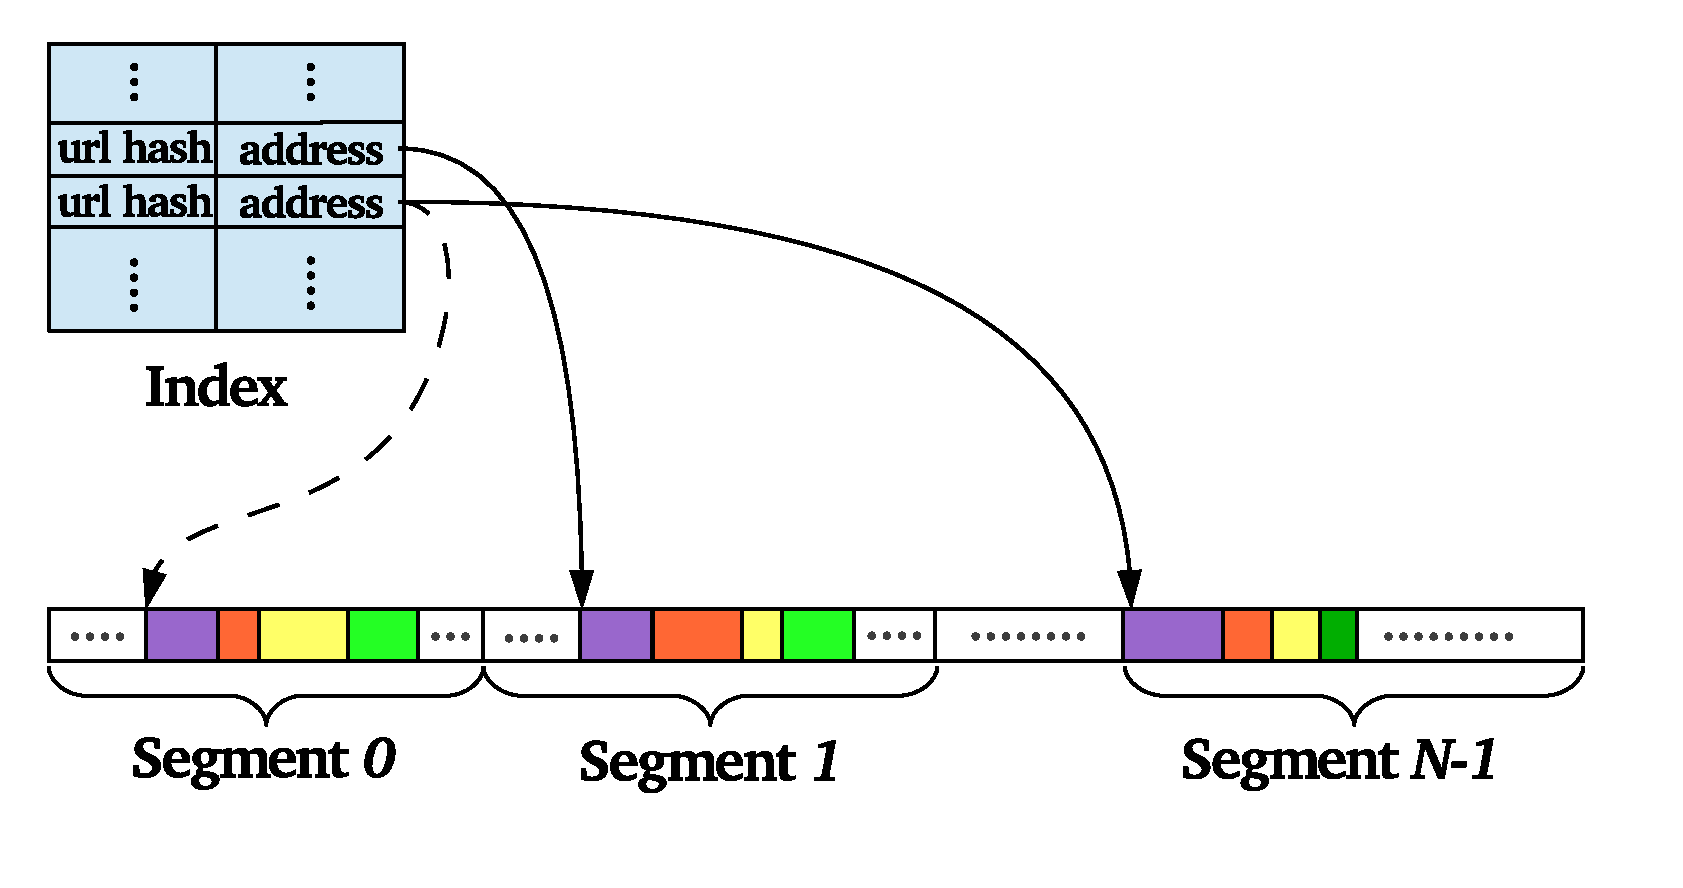
\includegraphics[width=1.04\columnwidth]{graphs/update}
  \end{center}
  \caption{Cache index and effect of updating an entry.}
  \label{fig:update} 
\vspace{-0.2in}
\end{figure}

\subsubsection{Update}
When an entry is updated (\emph{OpenEntry} $\rightarrow$ \emph{WriteData}, ..,
\emph{WriteData} $\rightarrow$ \emph{Close}), since we do not perform in-place
update, we write a completely new version of the entry to the write frontier.

Figure~\ref{fig:update} shows the effect of updating an entry.  An entry that
was originally written to \emph{segment 0} is re-opened for an update.  Once the
update is complete, the new version is written to the current write frontier,
\emph{segment n-1}.  It is possible that only part of the entry (e.g. one
stream) was modified; in this case, the remainder of the information is copied
from the old entry.

An alternative to copying unmodified streams is to store back pointers to the
original stream in the updated entry. This strategy was evaluated; the resulting
implementation gained very little in space savings at the cost of significant
complexity. In addition the loss of spatial locality led to a decrease in read
performance.

\subsubsection{Segment Life Cycle}
A segment starts in the \emph{free} state, goes to the \emph{current} state when
it is chosen as the write frontier, and eventually is filled and reaches the
\emph{closed} state.  A \emph{closed} segment is read-only until it is freed for
reuse.  Once the number of \emph{free} segments drops below a low watermark, a
cleaning process starts and frees segments until their number reach a high
watermark.

\begin{figure}[t]
  \begin{center}
    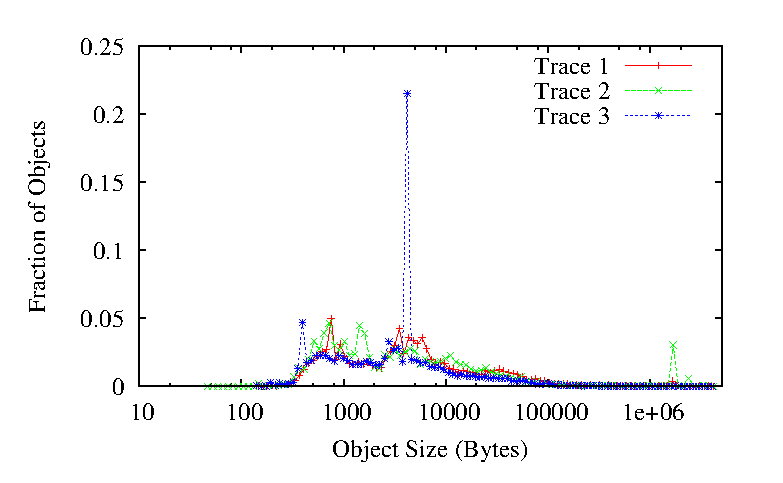
\includegraphics[width=1.04\columnwidth]{graphs/log-size-dist}
  \end{center}
  \caption{Log graph of object sizes in collected user traces.}
  \label{fig:log-size-dist} 
\vspace{-0.2in}
\end{figure}


\begin{figure}
  \begin{center}
    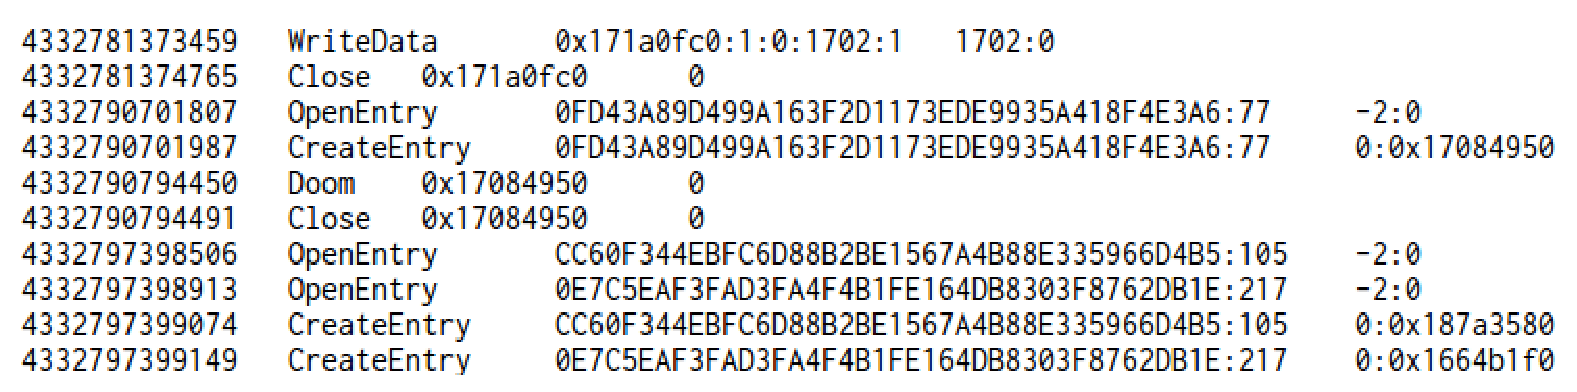
\includegraphics[width=\columnwidth]{graphs/trace}
  \end{center}
  \caption{Sample from a trace.}
  \label{fig:trace}
\vspace{-0.2in}
\end{figure}

\subsubsection{Cleaning a Segment}
Segments are chosen for cleaning in FIFO order, skipping any segments with
entries open for reading. Cleaning is done by reading the segment summary,
identifying the entries within the segment, and then for each entry retrieving
the entry key and checking whether the index for that key hash still points to
the entry. If not, the entry has been updated or deleted and no action is
required; if the index still points to this entry then it is active, and must be
evicted by removing its pointer from the index.

\section{Evaluation}

We implemented the log-structured cache for Chromium on Nexus 7, running Android
Jelly Bean 4.2.2 based on 3.4.x Linux kernel with ext4 file system.  In order to
evaluate it, we collected logs from a group of users who used an instrumented
version of the stock Chromium browser for two months as their main browser.  The
instrumentation logged arguments to the cache API in full detail, with URLs
hashed with random salts.  A short sample from a trace appears in
Figure~\ref{fig:trace}.

We note that these traces were collected on desktop and laptop systems (due to
Chromium not being completely open source on Android), and thus will differ from
mobile browser traces. In particular we expect the mean number of objects per
page to be fewer and the sizes of objects to be smaller.

\subsection{Storage Performance}

\begin{figure}
  \begin{center}
    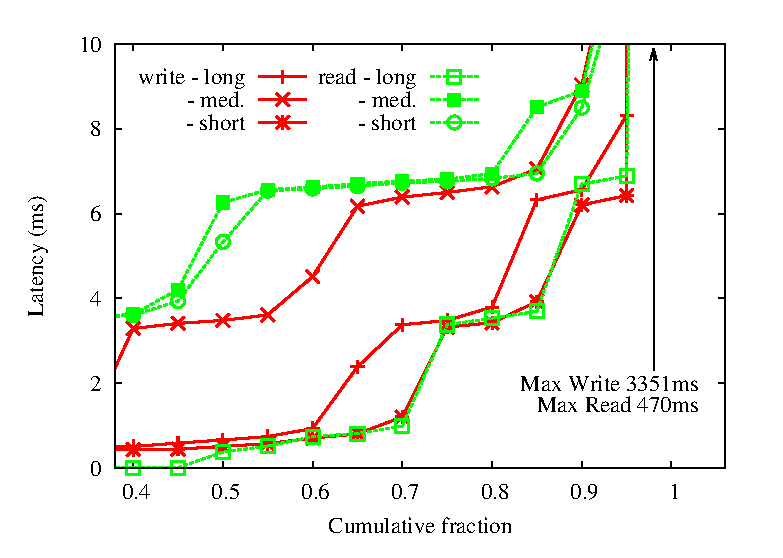
\includegraphics[width=1.04\columnwidth]{graphs/disk-perf}
  \end{center}
  \caption{ReadData and WriteData latency percentiles for the existing
    cache. Overall mean read = 3.05\,ms, write = 3.59\,ms.}
  \label{fig:disk-perf} 
\vspace{-0.2in}
\end{figure}

\begin{figure}
  \begin{center}
    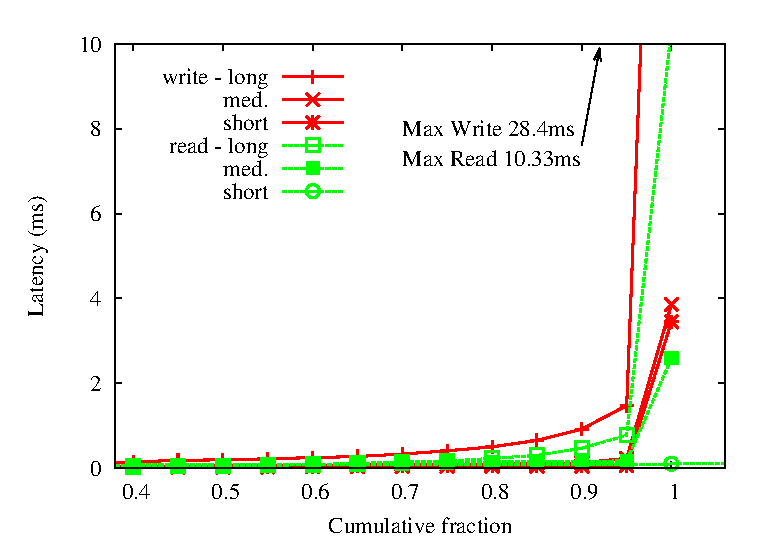
\includegraphics[width=1.04\columnwidth]{graphs/flash-perf}
  \end{center}
  \caption{ReadData and WriteData latency percentiles for the log-structured
    cache. Overall mean read = 0.148\,ms, write = 0.146\,ms.}
  \label{fig:flash-perf} 
\vspace{-0.2in}
\end{figure}

A test driver was used to replay and measure the latency of the operations. To
help ensure accurate reproduction of the application behavior it was
necessary to preserve inter-operation delays; when traces were
replayed at maximum speed, significant performance differences were
seen due to buffering and coalescing of operations at the file system
layer which did not occur in typical use. To reduce run-time these
delays were truncated to a maximum of 5 seconds, preserving most timing
within an individual browsing session while allowing weeks-long traces
to be replayed in less than a day.

Figure~\ref{fig:disk-perf} shows the CDF for \emph{ReadData} and
\emph{WriteData} operation latencies for the existing Chromium cache.  It can be
seen that the $95^{th}$ percentile \emph{ReadData} and \emph{WriteData} latency
is nearly 10ms, with a worst-case write latency of over 3 seconds.

Figure~\ref{fig:flash-perf} shows the corresponding data for the
\emph{log-structured cache}.  As can be seen, the $95^{th}$ percentile
\emph{ReadData} and \emph{WriteData} latencies are less than a millisecond, with
a worst case of 28 and 10ms.

\begin{table}[h]
{\footnotesize
\begin{tabular}{llrrrr}
\cline{2-6}
 &  & \multicolumn{4}{c}{Cache Size}                                                                                     \\ \cline{2-6} 
 &        & \multicolumn{1}{l}{1024 MB} & \multicolumn{1}{l}{512 MB} & \multicolumn{1}{l}{256 MB} & \multicolumn{1}{l}{128 MB} \\
 & Trace 1      & 1                           & 0                          & 0                          & 1                          \\
 & Trace 2      & 0                           & 0                          & 1                          & 1                          \\
 & Trace 3      & 0                           & 1                          & 0                          & 1                          \\ \cline{2-6} 
\end{tabular}
}
\label{table:collision}
\caption{Cleaning / object read collisions. A segment is skipped by the cleaner
  when an object in that segment is currently open for reading.}
\label{tab:skips}
\end{table}

\begin{figure}[t]
\centering
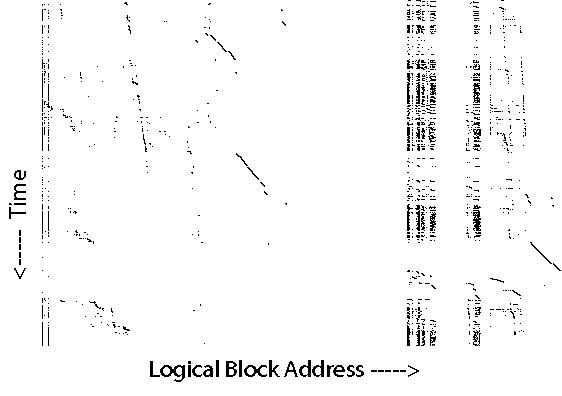
\includegraphics[width=0.8\columnwidth]{graphs/disk.png}
\caption{Block device access trace, original cache}
\label{fig:blktrace:disk}
\end{figure}

\begin{figure}
\centering
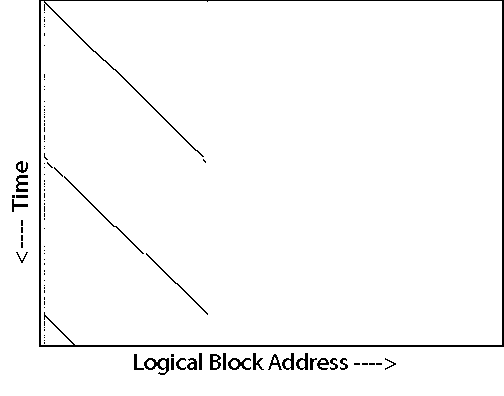
\includegraphics[width=0.717\columnwidth]{graphs/flash.png}
\caption{Block device access trace, log-structured cache}
\label{fig:blktrace:flash}
\end{figure}

\subsection{Hit Rate}

Hit rate was evaluated on the same traces used for testing storage
performance. First an upper bound on hit rate was established for each trace, by
simulating the operation of an \emph{infinite cache}.  That is, we instantiate a
cache large enough that would never evict an entry and then replay the trace on
it.  Since the traces were collected on a cache with bounded capacity, they
contain many failing \emph{OpenEntry} calls due to evictions, followed by an
immediate \emph{CreateEntry} call to insert the entry.  We fix these by
preprocessing traces and replacing such \emph{OpenEntry}-\emph{CreateEntry}
pairs with succeeding \emph{OpenEntry} calls, thus giving an impression of a
trace from an infinite cache.  With the \emph{infinite cache}, we never have a
failing \emph{OpenEntry} call with the exception of compulsory misses, giving an
upper bound on the hit rate.  For the collected traces this upper bound ranges
from 34\% to 45\%, which is consistent with previous studies~\cite{souders12}.

Due to maximum size limitation of 2\,GiB on the current Chromium cache, traces
were trimmed to ensure they did not exceed this size before further experiments
were performed.  In Figure~\ref{fig:hit-rate} we see the hit rate results for
the infinite cache case as well as the cache sizes ranging from 1\,GiB to
64\,MiB for both the original and the log-structured cache.
The impact on the hit rate is seen to be modest; in the worst case there is an
increase of 3\% in the miss rate, from 65\% to 68\%.

\begin{figure}[t]
  \begin{center}
    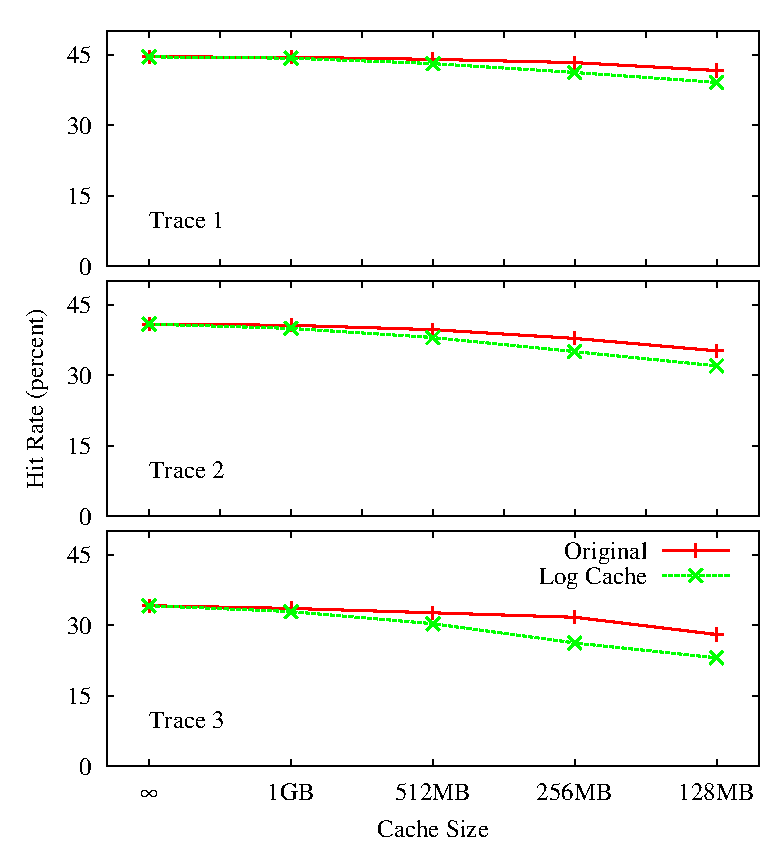
\includegraphics[width=1.04\columnwidth]{graphs/hit-rate-2}
  \end{center}
  \caption{Hit rate for the \emph{log-structured cache} with FIFO eviction
    policy.}
  \label{fig:hit-rate} 
\vspace{-0.2in}
\end{figure}

\begin{figure}
\centering
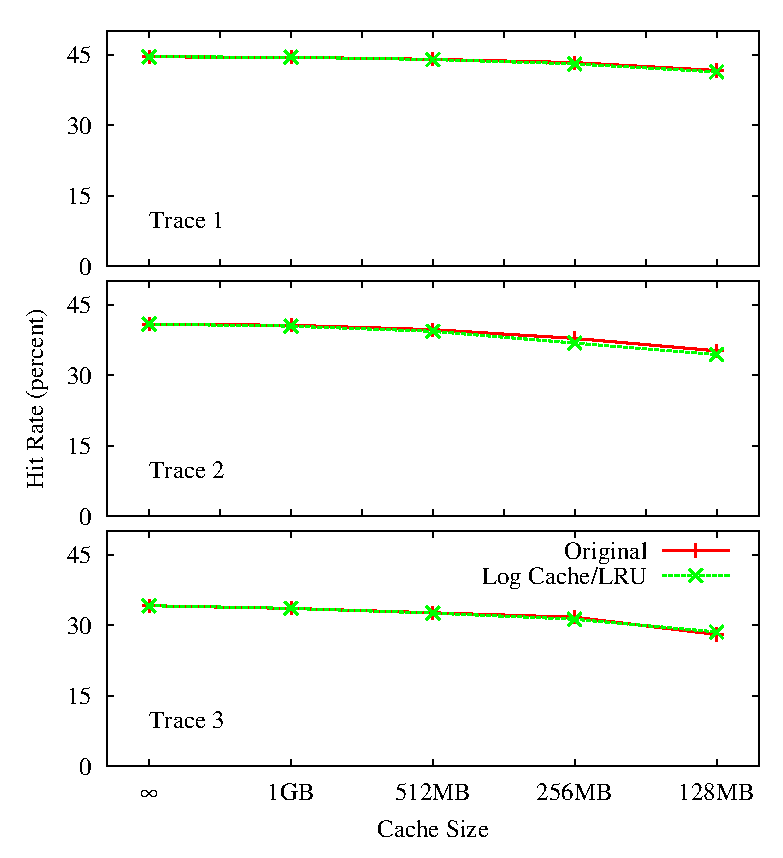
\includegraphics[width=1.05\columnwidth]{graphs/hit-rate-3}
\caption{Hit rate for the \emph{log-structured cache} with retention
  of recently-used objects during cleaning.}
\label{fig:hit-rate2}
\end{figure}

\subsection{Quantifying the Impact}
The reduction in per-operation overhead due to the log-structured cache will
result in a  performance improvement, while the decrease in hit rate will have
the opposite effect. We can quantify the effect of these two factors by noting
that the mean per-operation performance can be expressed as
\begin{equation}
T_{op} = T_{read}\cdot R_{hit} + T_{fetch}\cdot (1-R_{hit})
\end{equation}
where $T_{read}$ is the cache read operation latency, $R_{hit}$ is the hit rate,
and $T_{fetch}$ is the time to retrieve an object. For the original cache 
$T_{read}=3.05$ms, and we assume $R_{hit}=0.40$. Fetch time is $\frac{8\cdot S_{obj}}{R}$
where $R$ is the network speed in bits per second and $S_{obj}$ is the mean
object size in bytes.

For the log-structured cache, 
\begin{equation}
T_{op} = T_{read}'\cdot (R_{hit}-\Delta + T_{fetch}\cdot (1-R_{hit}+\Delta)
\end{equation}
where $T_{read}'=0.15$ms and we assume the reduction in hit rate, $\Delta$, is $0.5\%$. 
Assuming a mean object size of 10,000 bytes\footnote{Calculated from the
  measured traces} we find that at a network speed of
345\,Kbit/s the mean operation time will be equal for both caches; for
higher-speed connections (or smaller mean object sizes) the log-structured cache
will be faster. 
In other words, for modern wireless speeds the faster read performance
of the log-structured cache will far outweigh a small decrease in hit rate. 

We note that our assumed mean object size is determined from desktop
and laptop browsing measurements. It is likely that the mean object size will be
smaller on mobile devices, e.g. due to the inclusion of some fraction
of mobile-optimized sites; the resulting reduction in object fetch time will
further diminish the effect of a small hit rate reduction.
In addition, our analysis omits any consideration of writes, as they may
be performed in the background; however they have a significant (although
difficult to quantify) impact due to consumption of storage bandwidth and CPU
time needed by the critical-path portions of the application.

\section{Related Work}
A large body of work has examined the problem of caching web accesses at a proxy
providing service for large numbers of client users; an early survey of this
area is provided by Wang~\cite{wang_survey_1999}. Other work has focused more
specifically on cache replacement algorithms for web traffic
(e.g. Jelenkovi\'{c} and Radovanovi\'{c}~\cite{Jelenkovic_optimizing_2004}); a
survey by Podlipnig and B\"{o}sz\"{o}rmenyi ~\cite{podlipnig_survey_2003} covers
many such algorithms which have been proposed. Unlike our work, which focuses on
the per-operation cost of the browser cache, web proxy research has in general
focused on abstract performance---i.e. byte or object hit rates---and assumed
that a sufficiently powerful server would be deployed to handle the workload.

A number of researchers have recently begun to investigate mobile browser cache
performance. Qian et al. at Michigan~\cite{qian_web_2012} have analyzed data
collected by a cellular provider, as well as additional user-contributed traces,
measuring cache effectiveness; their results show that as much as 20\% of mobile
browsing traffic is redundant and could be avoided by better caching. Wang et
al. \cite{wang_how_2011} examine per-user traces and analyze top10 websites,
finding that revalidation traffic hampers cache performance in high-latency
mobile environments. In each case the focus has been on the cacheability of data
in the mobile environment, rather than the system performance of cache
operations.

Most recently Kim et al. \cite{kim12} have examined the effect of storage
devices on performance of mobile applications. Their work found that in many
cases the limiting factor in performance, even for high network traffic
applications like browsing, was the poor performance of flash storage devices
rather than limited network bandwidth. Our work is motivated by this
investigation, and extends their work to examine a specific application, web
browsing, where significant changes may be made to optimize storage behavior.

Finally, although the idea of a log-structured cache is not new, we have not
found it presented and examined in the academic literature.  Badam et
al. ~\cite{hashcache} mention a commercial caching product based on a
log-structured design, yet they explicitly mention that the product website has
disappeared and there are no citable references.

\section{Conclusions}

Analysis of caching implementations all too often focus exclusively on
counting hits and misses, ignoring the question of how fast the
resulting system runs. In contrast our cache for the Chromium browser
is designed to maximize the performance of the hit and miss operations
themselves, speeding them up by almost an order of magnitude, at the
cost of a modest reduction in hit rate. Further work will focus on
quantifying the actual impact on user-visible performance, as well as
investigating whether hit rate may be improved without significantly
impacting storage performance.

\section*{Acknowledgments}

We would like to thank Ricardo Vargas of Google Chrome team for answering our
questions related to Chromium disk cache and helping us with performing
experiments on Chromium's existing cache.

\bibliographystyle{acm}
\bibliography{sigproc}  % sigproc.bib is the name of the Bibliography in this case

\end{document}
